\documentclass[a4paper]{jpconf}
\usepackage{graphicx,amsmath}
\bibliographystyle{iopart-num}

\begin{document}
\title{Upgrades to the SINQ Cold Neutron Source}

\author{R M Bergmann, U Filges, D Kiselev, T Reiss, V Talanov and M Wohlmuther}

\address{Paul Scherrer Institut, 5232 Villigen, Switzerland}

\ead{ryan.bergmann@psi.ch}

\begin{abstract}Changing the configuration of the cold neutron source during an extended shutdown of Swiss Spallation Neutron Source (SINQ) is being considered for improving performance of the instruments that use the cold source.  The cold neutron source consists of a 20 L volume of liquid D$_2$ at approximately 25 K.  Previous upgrades included adding a re-entrant hole into one side of the D$_2$ volume to allow cold neutrons to stream uninhibited from the center of the source towards the instrument neutron guides.  Calculations done prior to these changes predicted cold neutron fluence gains from 1.2 to 1.6, with gains increasing with wavelength. These increases have not been observed, and it is suspected that the re-entrant hole is not fully voided.  Voiding the re-entrant hole relies on radiative heating to boil D$_2$ which in turn fills the re-entrant hole cavity, pushing the liquid D$_2$ out.  Proposed plans include making the re-entrant hole external (ensuring that it is not filled with liquid D$_2$), removing some extra structural material around the D2 tank, redesigning the re-entrant hole geometry to be more optically ideal, introducing a Pb-208 reflector to minimize cold neutron up-scattering from the surrounding D$_2$O moderator tank, and implementing a small liquid H$_2$ volume to provide a cold neutron “hot spot” for certain instruments.  These changes are predicted to increase neutron fluence between 1.1 to 2.0 times the current levels, depending on instrument location, view, and wavelengths of interest.
\end{abstract}

\ack{This work was supported by Swiss National Science Foundation grant 200021\_150048/1.}

\section{Introduction}

There is a planned shutdown of the Swiss Spallation Neutron Source (SINQ) in 2017, which provides an opportunity for changes to be made to the liquid deuterium cold neutron source.  The 20 liter volume of liquid D$_2$ at approximately 25 K is located within the D$_2$O moderator tank surrounding the Pb spallation target.  The innermost face of the cold source is approximately 35 cm away from the center of the target.  In the planned upgrade strategies, no changes to the surrounding aluminium and zirconium safety hulls will be made, and no changes to the insert tube structure will be made.  I.e., all changes must fit into the existing multi-walled insert geometry.  

\section{Re-entrant Hole}

The goal of the re-entrant hole (REH) is to remove scattering and absorbing material between the cold neutron maximum and the direction of interest.  In this case, the cold neutron maximum is at the center of the cold source and the direciton of interest is towards the SINQ guide hall.  

Voiding the re-entrant hole relies on radiative heating to boil D$_2$ which in turn fills the re-entrant hole cavity, pushing the liquid D$_2$ out.  Proposed plans include making the re-entrant hole external (ensuring that it is not filled with liquid D$_2$)

Calculations done prior to these changes predicted cold neutron fluence gains from 1.2 to 1.6, with gains increasing with wavelength. These increases have not been observed, and it is suspected that the re-entrant hole is not fully voided.  All future designs will have an external REH, which will decouple the fill level from radiation heating and ensure that the REH is never filled with liquid D$_2$.

\section{Simulation Geometry}

Figure \ref{geom} shows a zoomed-in view of the important parts of the MCNP model geometry.  A CAD model of the neutron guide bundles was converted to MCNP geometry by the MCAM software from XXX university in XXX China and integrated into the model \cite{mcam}.  The target is made of Pb rods with zircalloy cladding and is cooled by D$_2$O, the moderator tank is filled with D$_2$O, the cold source is liquid D$_2$, the nozzles with a low-pressure helium mixture, and the shielding and neutron guide structure is steel.  All structural material in the moderator tank is AlMg3, which is shown in yellow in Figure \ref{geom}.

\begin{figure}
\begin{center}
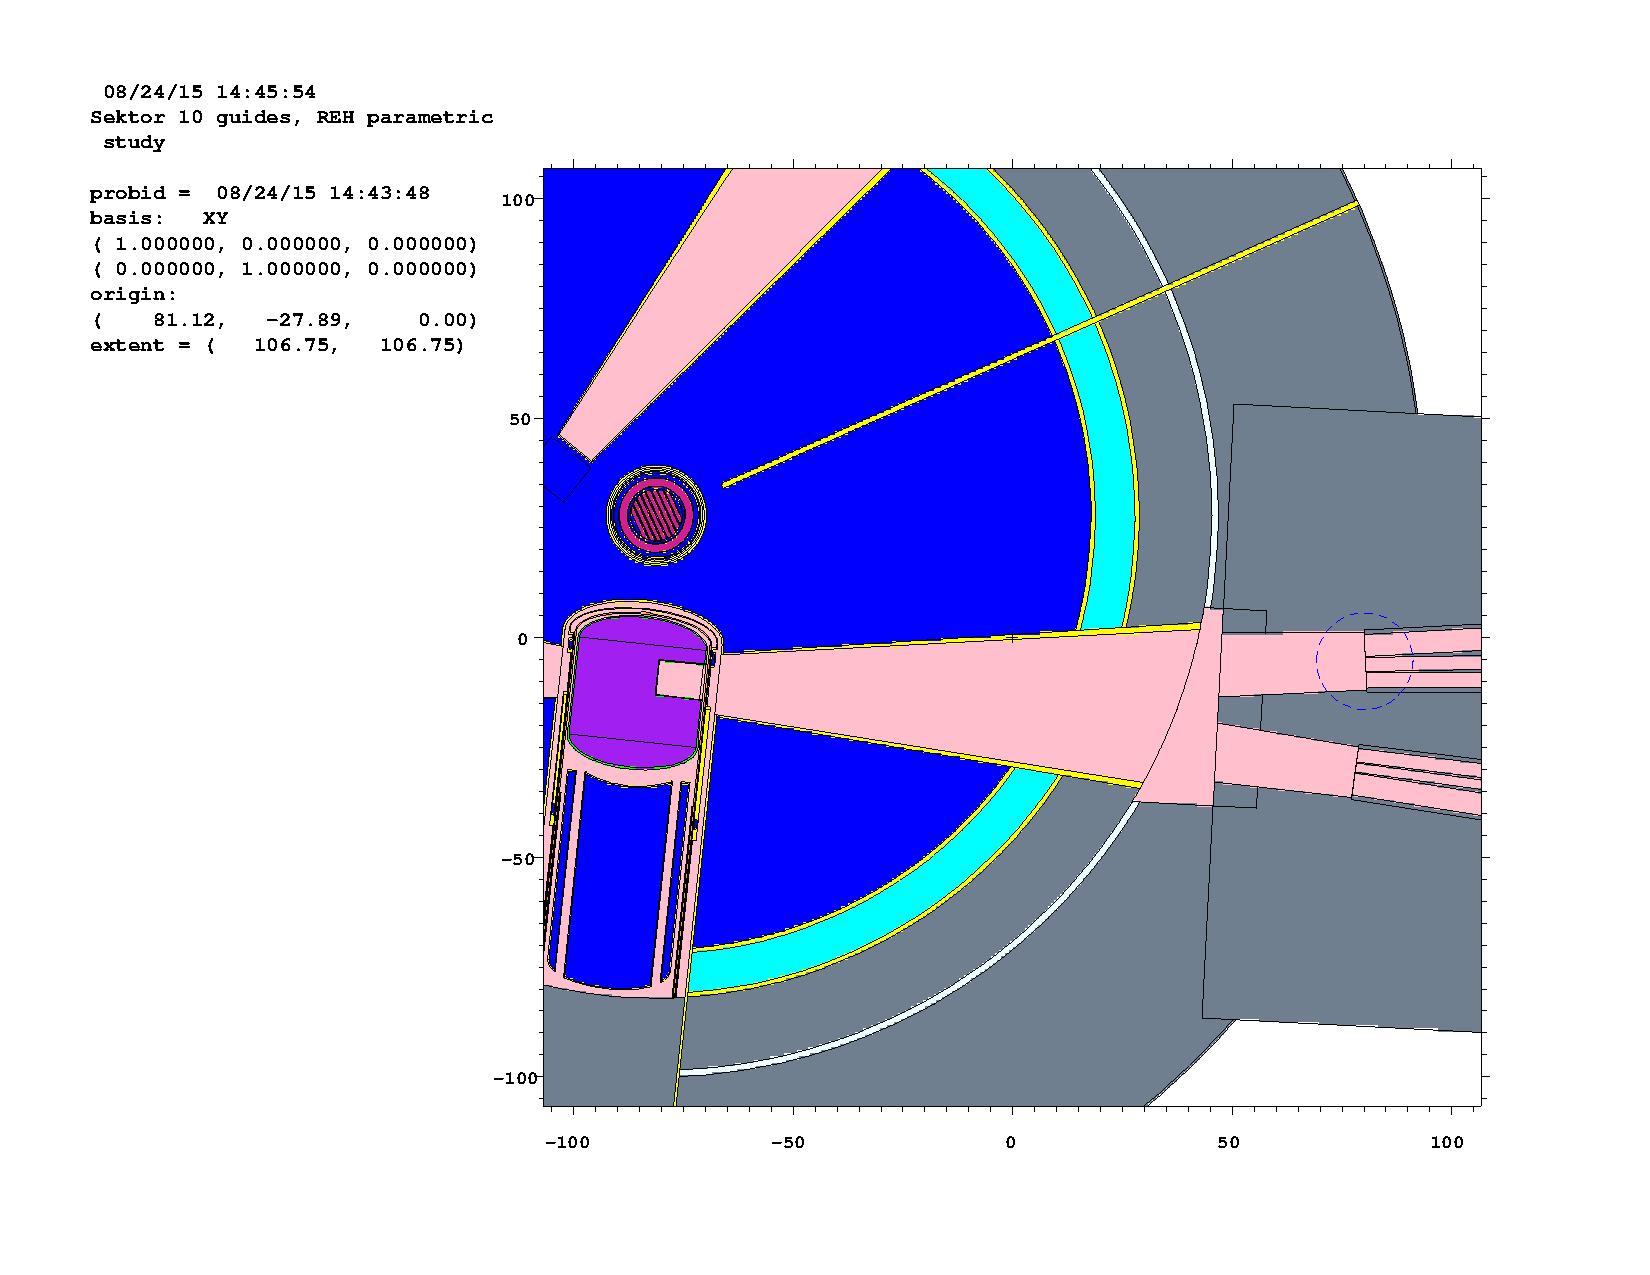
\includegraphics[trim={9.2cm 8cm 4cm 8cm},clip]{graphics/geom.pdf}
\end{center}
\caption{\label{geom}A horizontal slice through the MCNP simulation geometry showing the target (magenta), moderator tank (blue), cold source (purple), nozzle (pink), and neutron guide entrance (grey with circle).}
\end{figure}

\section{Variance Reduction}

Two variance reduciton methods were used in conjunction in order to perform the calculations in a reasonable amount of time.  First, mesh-based weight windows were generated based on the response of a point detector located 75 cm from the neutron guide entrance.  These windows serve to increase the number of neutrons that scatter inside the cold source while preserving the mean particle weight of an analog simulation by casusing the neutrons in the moderator tank to carry a higher weight then be split into many lower-weight particles when they enter the cold source volume.  

The second variance reduction method used is a ``DXTRAN'' sphere.  This tool is a non-physical sphere that is placed around the guide entrance that causes neutrons to be generated on its surface.  Whenever a neutron undergoes a scattering reaction, the probability of scattering into the sphere's direction is calculated, a line is traced from the scattering location to the sphere's surface, and a neutron is generated there with a weight reduced by the scattering probability and the optical thickness of the medium in between.  The generated neutrons are then transported normally inside the sphere \cite{mcnp}.  This method served to preferentially scatter neutrons into the direction of the neutron guide.

\section{Neutron Guide Response} 

In conjunction with the variance reduction methods described in the previous section, an approximation to how the neutron geuides transport neutrons was also used.  A patch was developed at ORNL and PSI that implements the McStas guide reflectivity model in MCNPX 2.5.0 and 2.7.0 \cite{mcnp_reflectivity, EK_reflectivity}, but the model is analog and is not fully compatible with DXTRAN spheres.  The implmentation is analog in the sense that if a neutron is sampled to \emph{not} reflect on a guide surface, it is transmitted into the next cell.  This means that neutron paths have to be sampled multiple times to account for any reflectivity losses, which slows the simulation down.  

Also, some stability issues were encountered while using the reflectivtity patch in conjunction with the DXTRAN sphere.  In order to ensure stable runs, a simulation was done first where a surface source was written at the guide entrance surface where any neutrons entering the guide were recorded and terminated.  This source was used in a second simulation with the guide reflecitvity turned on and used to transport the entering neutrons to the end of the guide where a tally was scored.  Again, this process slowed the simulation down and made studies with many cases more difficult.  An approximaiton to the guide response was used to eliminate the need for a second run to simply get the neutrons to the end of the guide.


\subsection{Guide Reflectivity}

The guide reflectivity model implmented in MCNP is identical to that used in McStas.  The reflectivity curve for the current guide in the SINQ hall is shown in Figure \ref{SINQ_reflectivity} andh the reflectivity equation and parameter values shown in Eq. \ref{eq:ref}.  The values shown are the same for all the guides in the SINQ hall \cite{SINQ_guide_values}.

\begin{figure}[h]
\begin{minipage}{14pc}
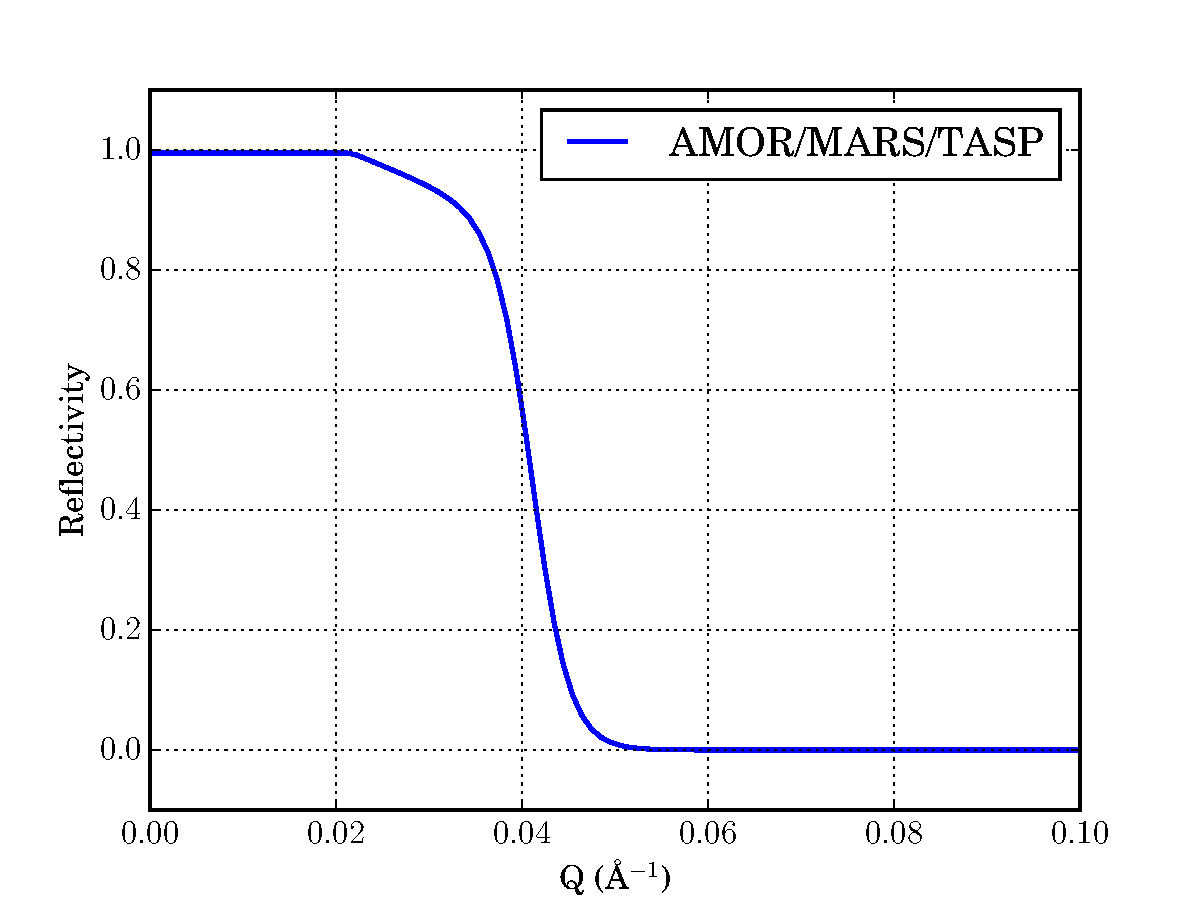
\includegraphics[scale=.4]{graphics/refl.pdf}
\caption{\label{SINQ_reflectivity} The reflectivity curve of the current SINQ neutron guides.}
\end{minipage}\hspace{5pc}%
\begin{minipage}{11pc}
\begin{multline}\label{eq:ref}\scriptsize
R(Q) = 
\begin{cases}
    \mbox{if } Q > Q_c : \\
    \frac{R_0}{2}\left\{  1 - \tanh\left(  \frac{Q - m Q_c}{W}\right) \right\}\{1-\alpha(Q-Q_c)\} \\
    \\
    \mbox{if } Q \leq Q_c :\\
    R_0 \\
\end{cases} \\ \\ \\
\begin{tabular}{c c c}
$R_0=0.995$ & $Q_c=2.17\times10^{-2}\AA^{-1}$ & $m=1.9$ \\ 
$\alpha=6.40 \AA$ & $W=4.0\times10^{-3} \AA^{-1}$ 
\end{tabular} \\
\end{multline}
\end{minipage} 
\end{figure}

Since the neutron reflection probability is based on momentum transfer and the reflections are specular, it is determined by the incident neutron angle and energy.  If the guide is rectangular, the reflection probability will not change as the neutron travels down the guide since the reflection angle will remain constant.  These conditions mean that the exiting neutron current should be compleltely defined by the incident polar angle and energy of a neutron entering the guide.  The position in the guide entrance will determine the phase of the exiting rays, but if the entire exit surface is summed over, this phase becomes irrelevant.

\subsection{Reconstruction}

In order to approximate the neutron current exiting the guide, a number of fixed-source runs of MCNPX were done as precalculations to the parametric study.  An evenly-distributed source was defined at the entrance surface of the guide that emits neutrons in a polar angle bin $1/8^\circ$ wide and logarithmically in energy (to ensure low energies are sampled fairly).  The exiting current at the end of the guide was tallied and divided by the entrance current to yield a transfer function in energy for the polar angle of the source.  This was done for $0-7.5^\circ$ of polar angle to yield the set of 60 functions shown in figure \ref{xfer_func}.  The colors mean????

%trim <left> <lower> <right> <upper>
\begin{figure}
\begin{center}
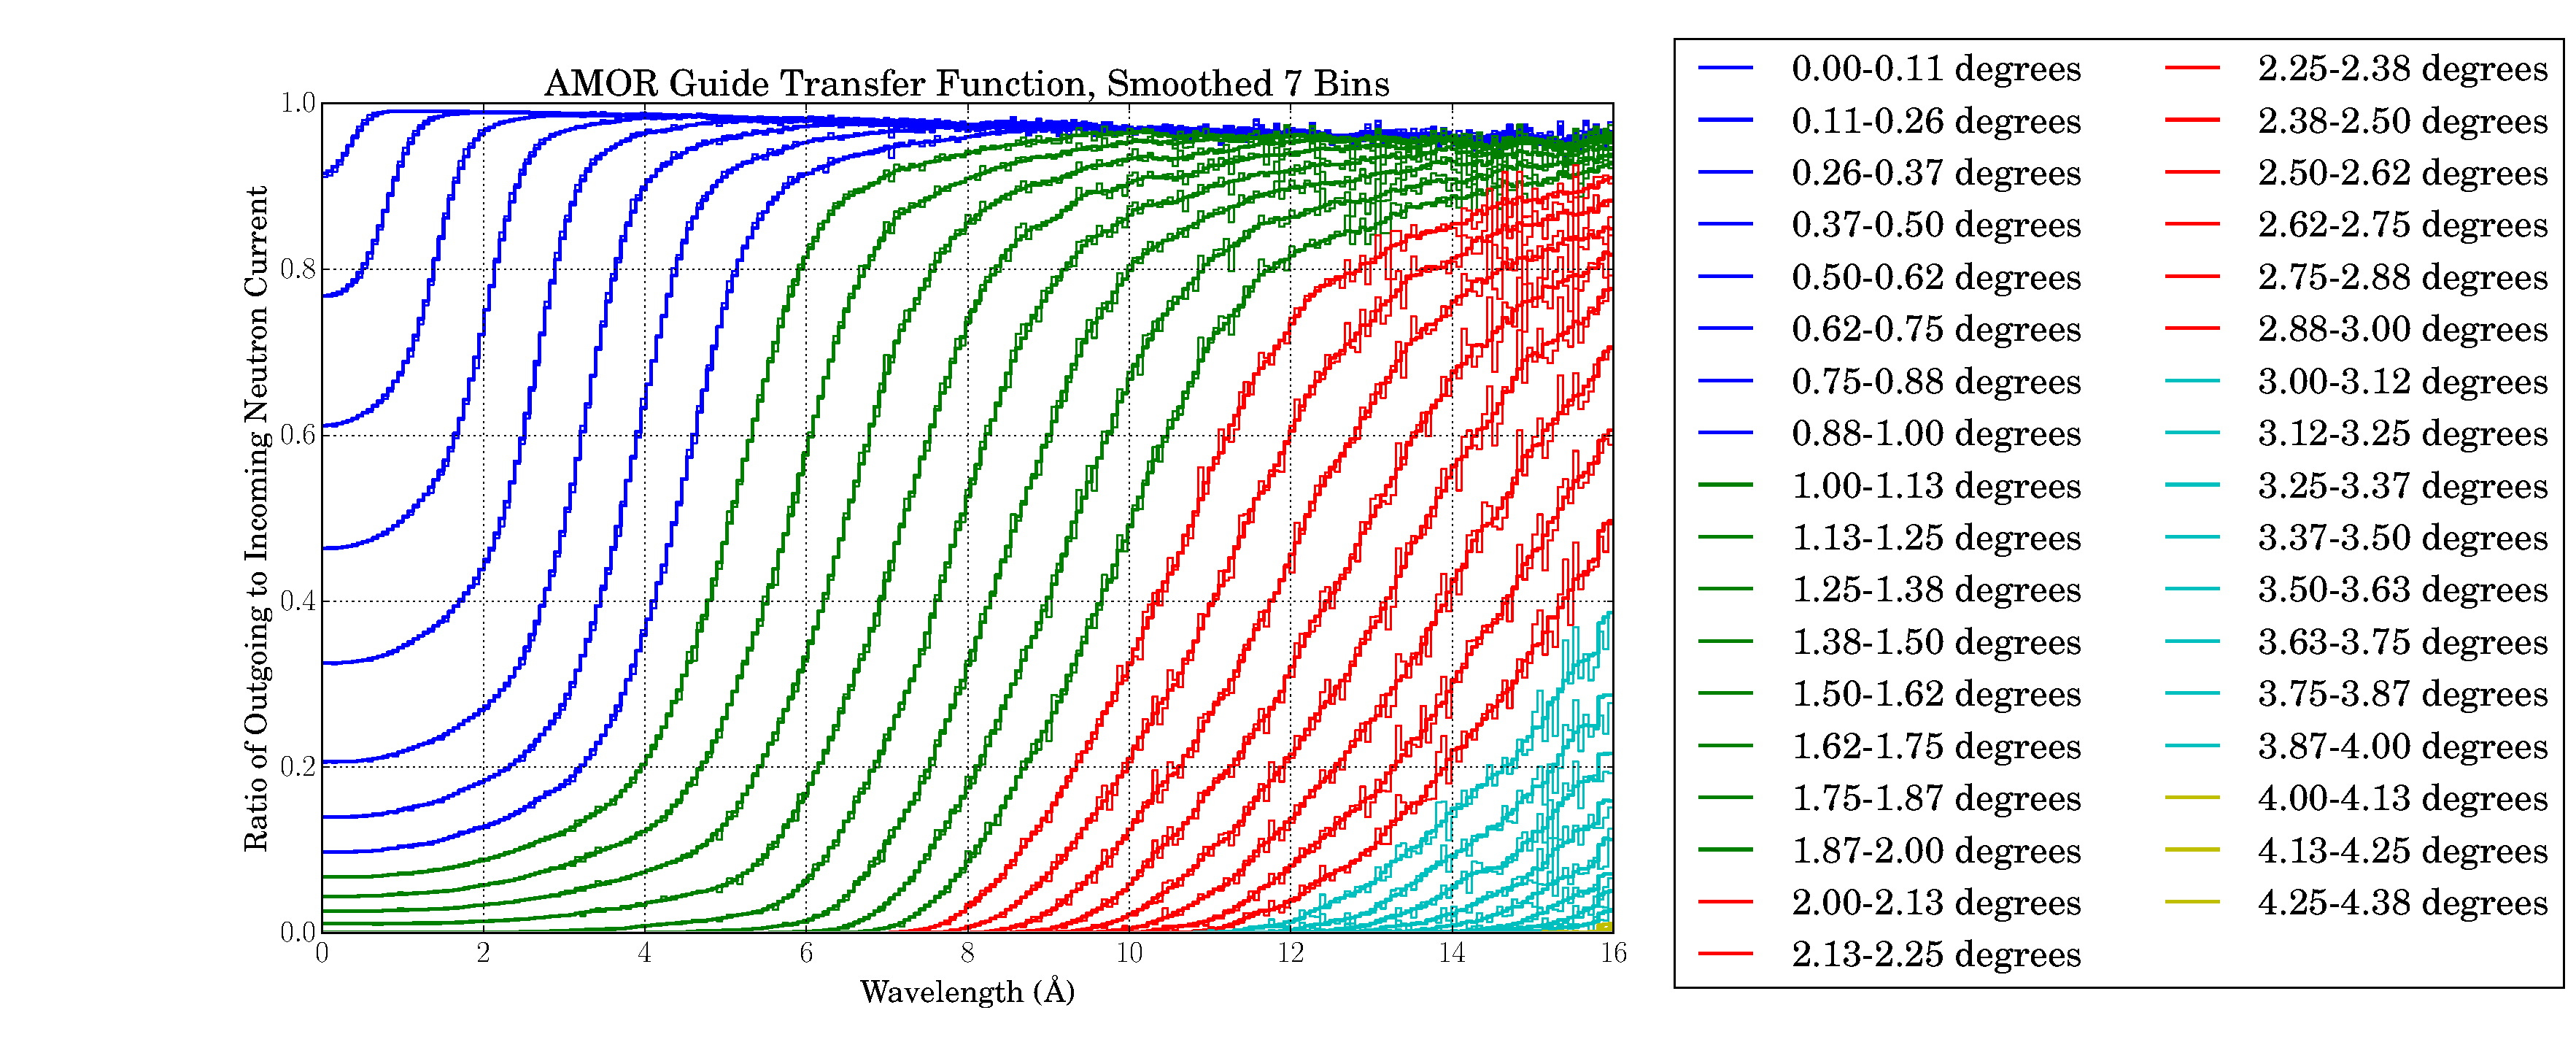
\includegraphics[scale=0.3,trim={2cm 1.7cm 2cm 0.8cm},clip]{graphics/xfer_func.pdf}
\end{center}
\caption{\label{xfer_func}Set of transfer functions for a m=2 guide.}
\end{figure}

If neutrons are tallied at the guide entrance in the same polar and energy binning as the transfer funcitons, it can be multiplied by the set and summed over all incident angles to yield the integrated neutron spectrum at the guide exit.  This way, the reflectivity model can be eliminated from the transport runs and a good estimate of the exiting current can still be made.

\subsection{Self-Consistency Test}

In order to verify that the reconstruction method works as expected, a comparison to the spectrum calculated by the explicit model was made.  As mentioned previously, a surface source was written at the guide entrance, then this was used as the source for a second run with the guide reflectivity activiated.  During this run, the entry and exit current was tallied.  The entry current was binning in polar angle according to the divisions in the pre-calculated transfer functions.  The results of the comparison are shown in Figure \ref{xfer_bench}.  The green line is the integrated neutron spectrum at the guide entrance, the blue line is the integrated exit current that was tallied at the guide exit, and the red curve is the exit spectrum calculated by multiplying the entrance spectrum by the transfer functions (and then summing them).  The maximum error seen is about XXX\%, and decreases with energy, and has a 1-norm value of XXX\%.

\begin{figure}
\begin{center}
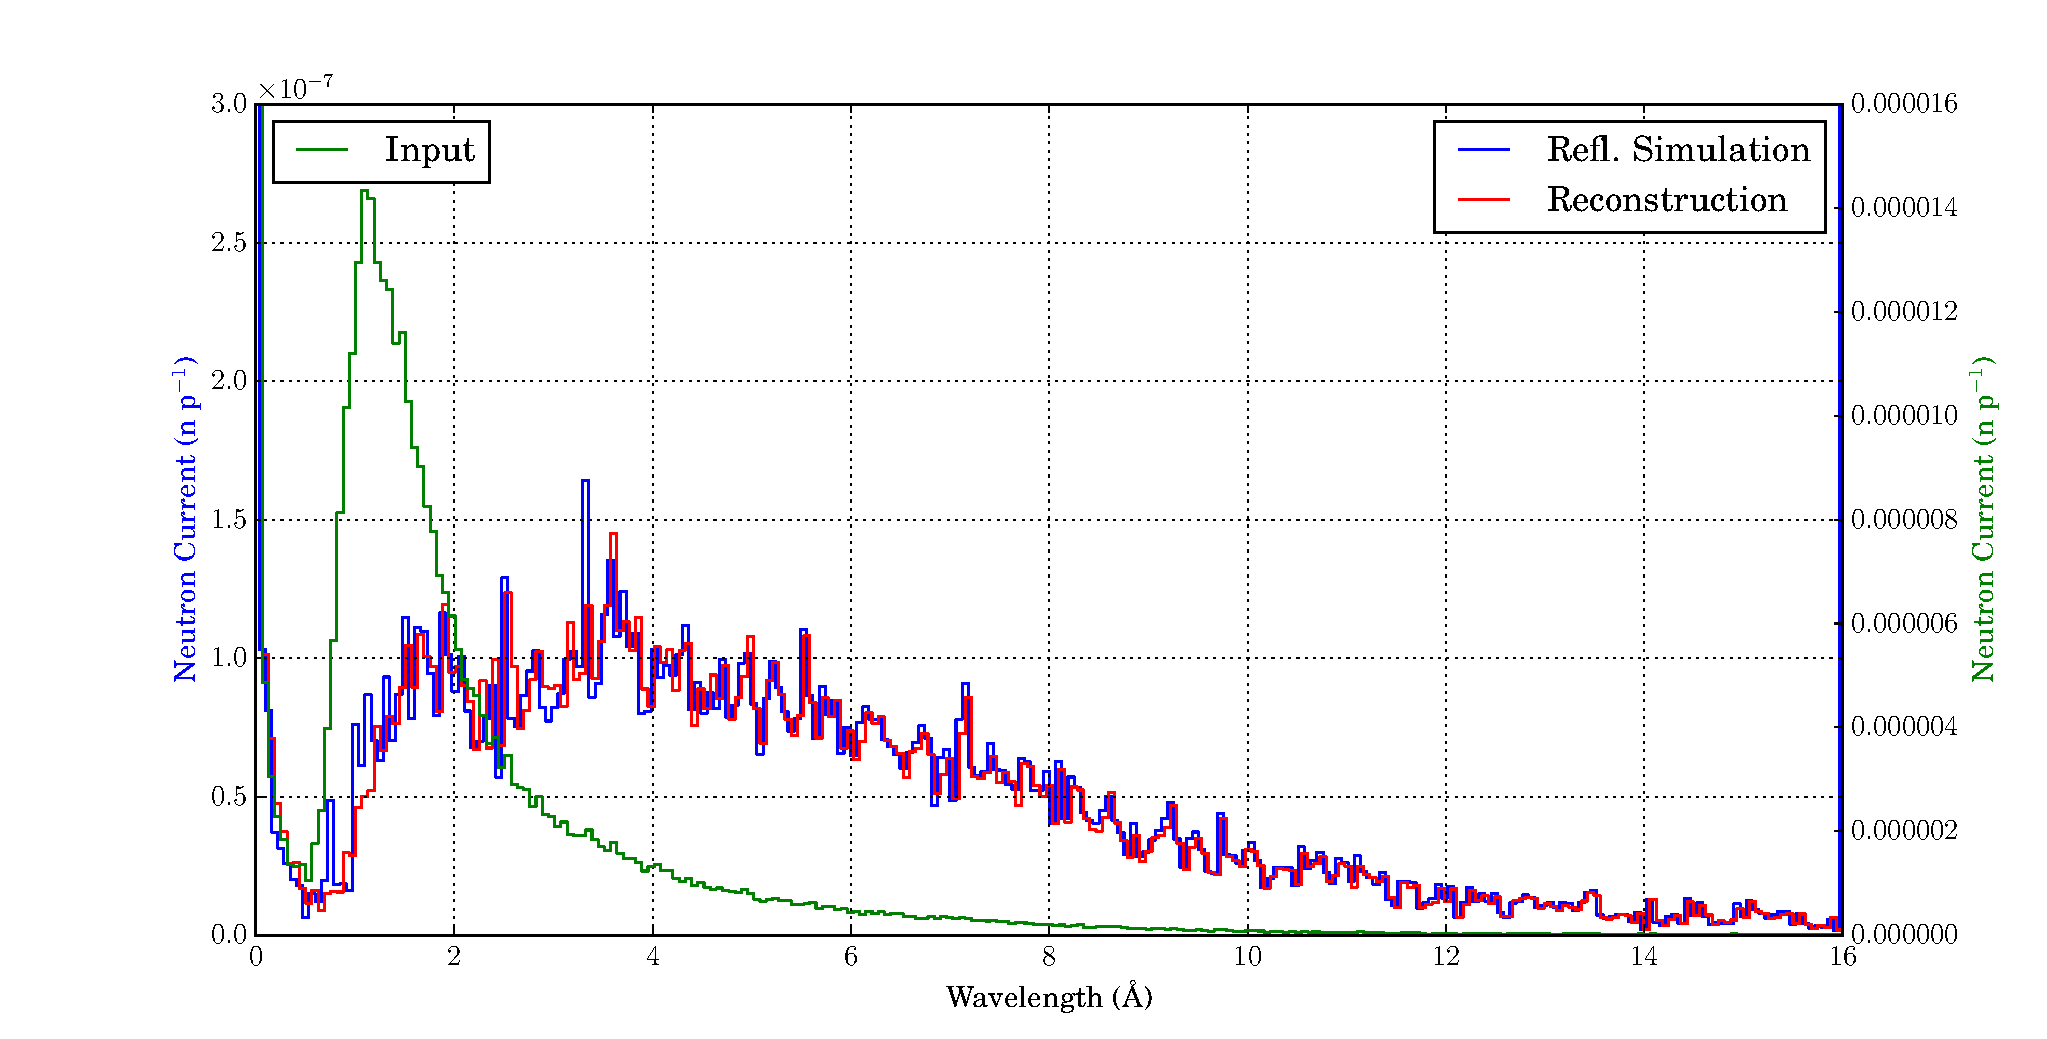
\includegraphics[scale=0.4]{graphics/xfer_bench.pdf}
\end{center}
\caption{\label{xfer_bench}The reconstructed guide exit current compared to the exit current calculated with a MCNP simulation with guide reflectivity activated.}
\end{figure}

\section{REH Parametric Study in the Horizontal Plane}

The re-entrant hole parametric study was done to investigate a wide range of geometries in the horizonal plane, where the guide width is smaller than the hole size.  Four REH depths (14, 10, 6, 2 cm), four opening widths (4, 8, 12, 16 cm), and eleven hole slopes (-0.5, -0.4, -0.3, -0.2, -0.1, 0.0, 0.1, 0.2, 0.3, 0.4, 0.5) were investigated in the study for a total of 176 cases. Figure \ref{parametric_geom} shows the parameters in relation to the cold source geometry.  The REH vertical dimensions were chosen to be the full width of the nozzle with a slight tapering slope inward.  The vertical dimensions were kept constant in this study, but will be the focus of future work.

\begin{figure}[h]
\begin{minipage}{14pc}
\begin{center}
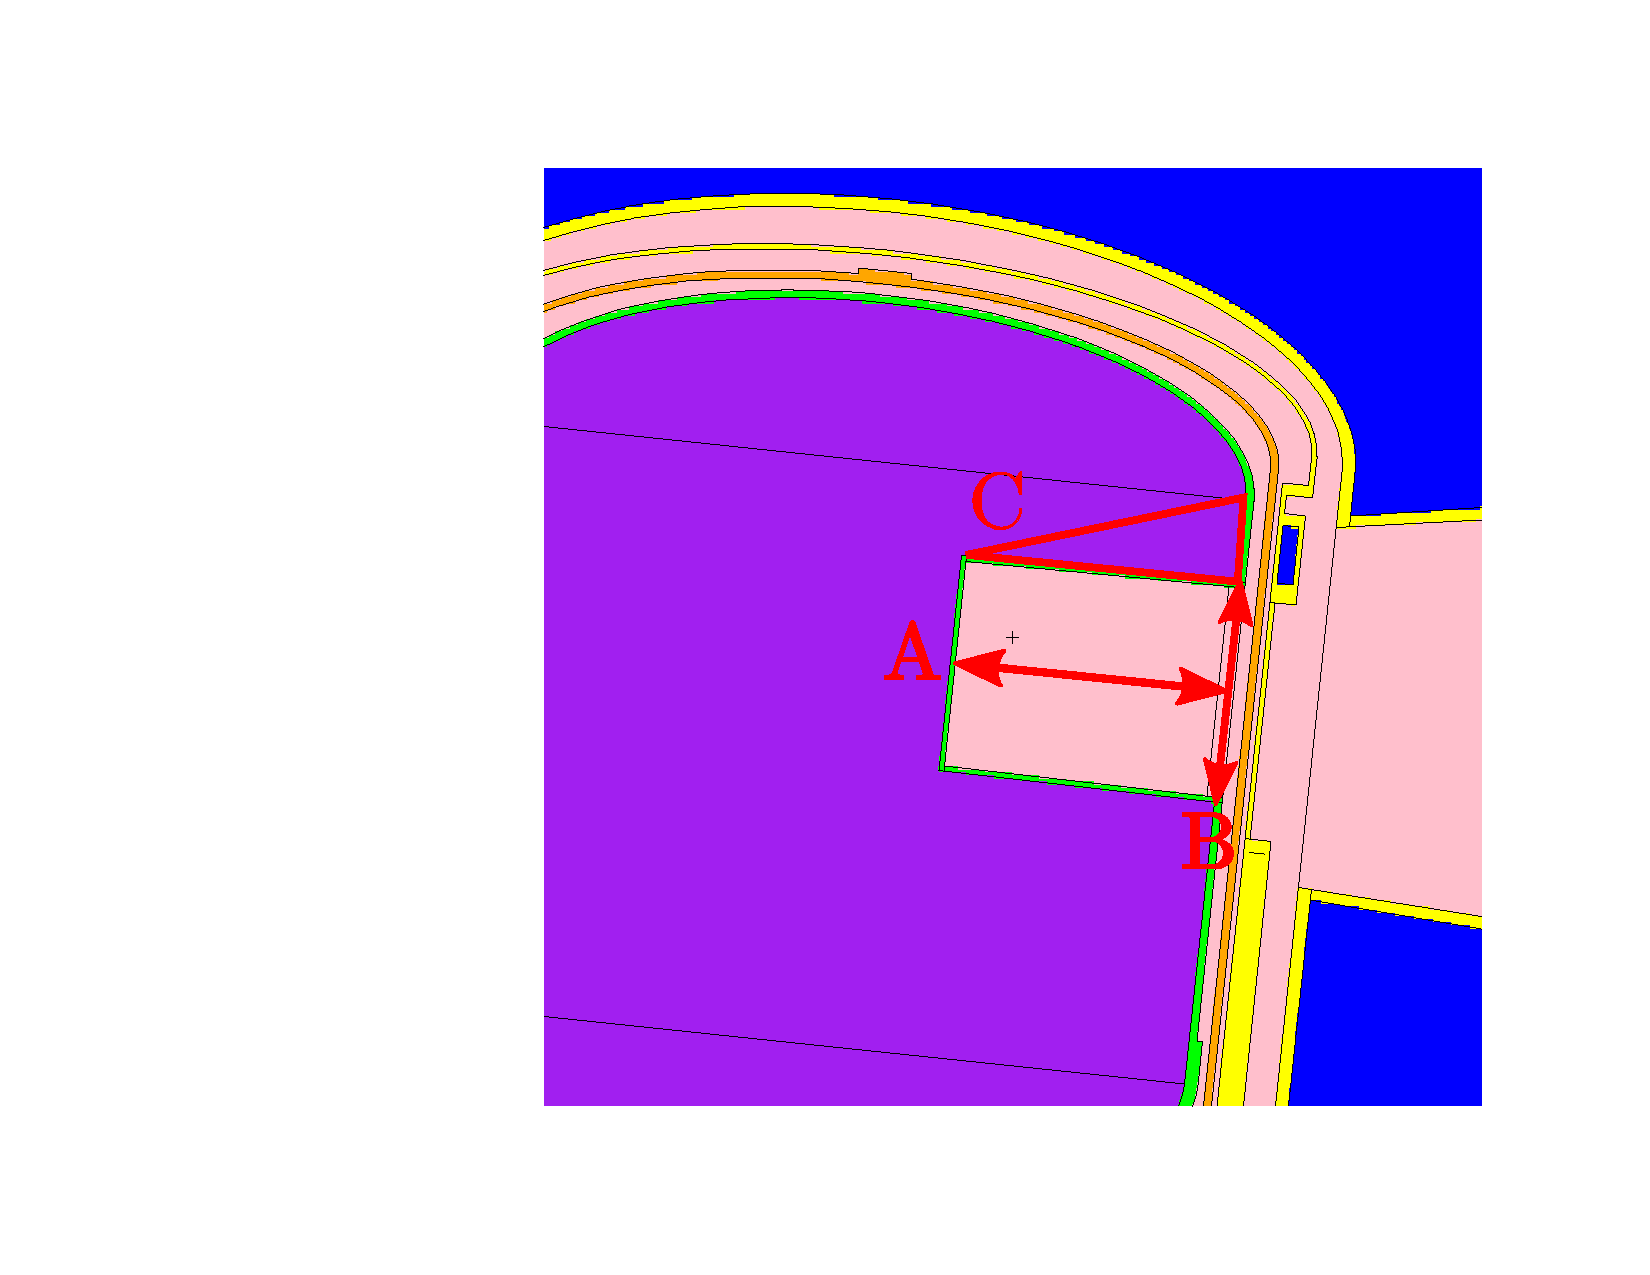
\includegraphics[scale=0.4,trim={13cm 6cm 4cm 5cm},clip]{graphics/para_geom.pdf}
\end{center}
\caption{\label{parametric_geom}The geometry varied in the REH parametric study. ``A'' is the hole depth, ``B'' is the opening width, and ``C'' is the hole slope.}
\end{minipage}\hspace{5pc}%
\begin{minipage}{11pc}
\begin{center}
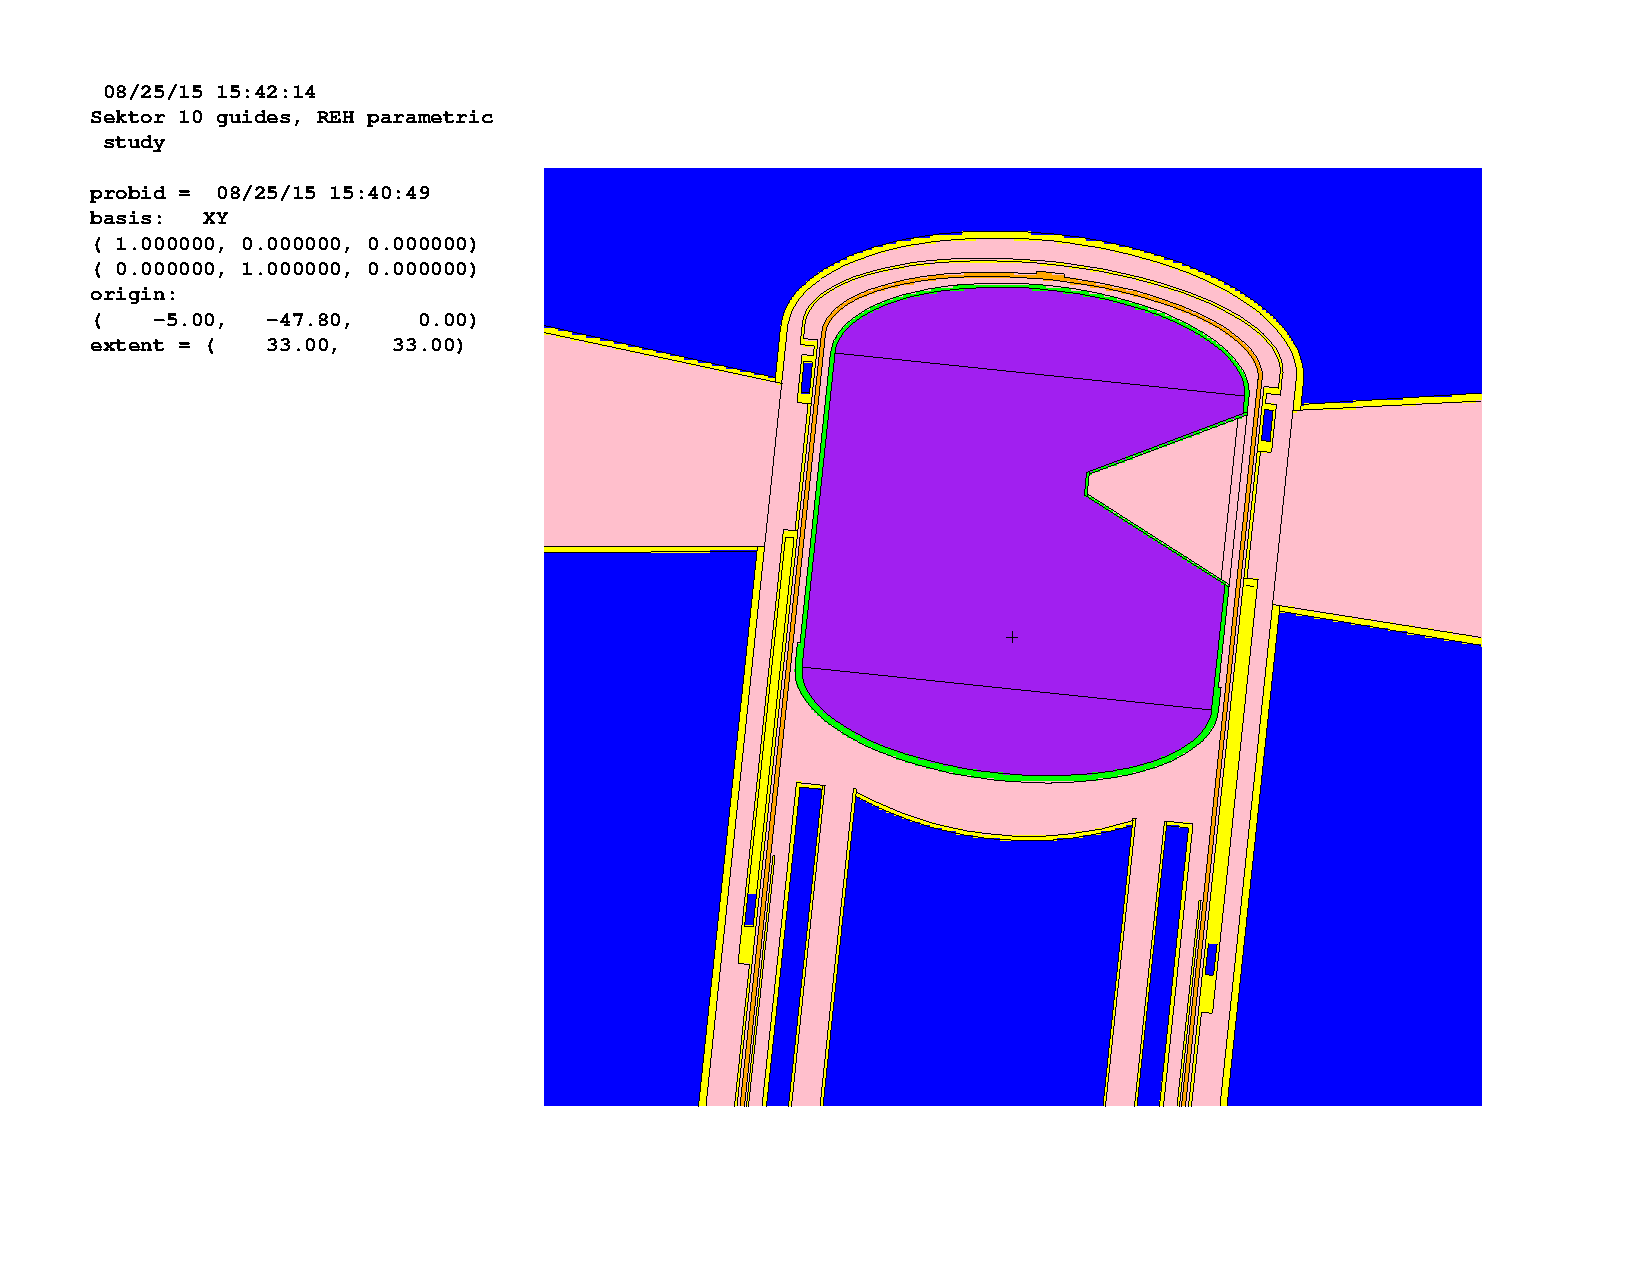
\includegraphics[scale=0.4,trim={11.2cm 8cm 5cm 3cm},clip]{graphics/case077.pdf}
\end{center}
\caption{\label{case077}The best-performing horizontal geometry for the REH.}
\end{minipage} 
\end{figure}

With all of the variance reduciton and approximations implemented, each case took about one hour to run on a 144-core configuration on a computer cluster at PSI.  The spectra from all the cases are shown in upper plot in Figure \ref{parametric_REH}, and their figures of merit are shown in the lower plot.  The figure of merit was chosen to be the total current exiting the guide from 3 to 6 \AA{} -- the wavelength band which is useful for most of the instruments in the guide hall.  The parameters were varied in slope-width-depth order, with slope being the fasted varied parameter. Figure \ref{parametric_REH} has labeled, colored blocks in the lower plot to show which parameters are constant for that block.  Slope and opening width have the most affect on performance at large depths.

The geometry of the best-performing case is shown in figure \ref{case077}.  The depth is 10 cm, the opening width is 12 cm, and the slope is 0.5.  This opening is as wide as the nozzle and almost tapers to a point at the maximum depth.  The maximum depth is 4 cm from the radial center of the cold source.  

\begin{figure}
\begin{center}
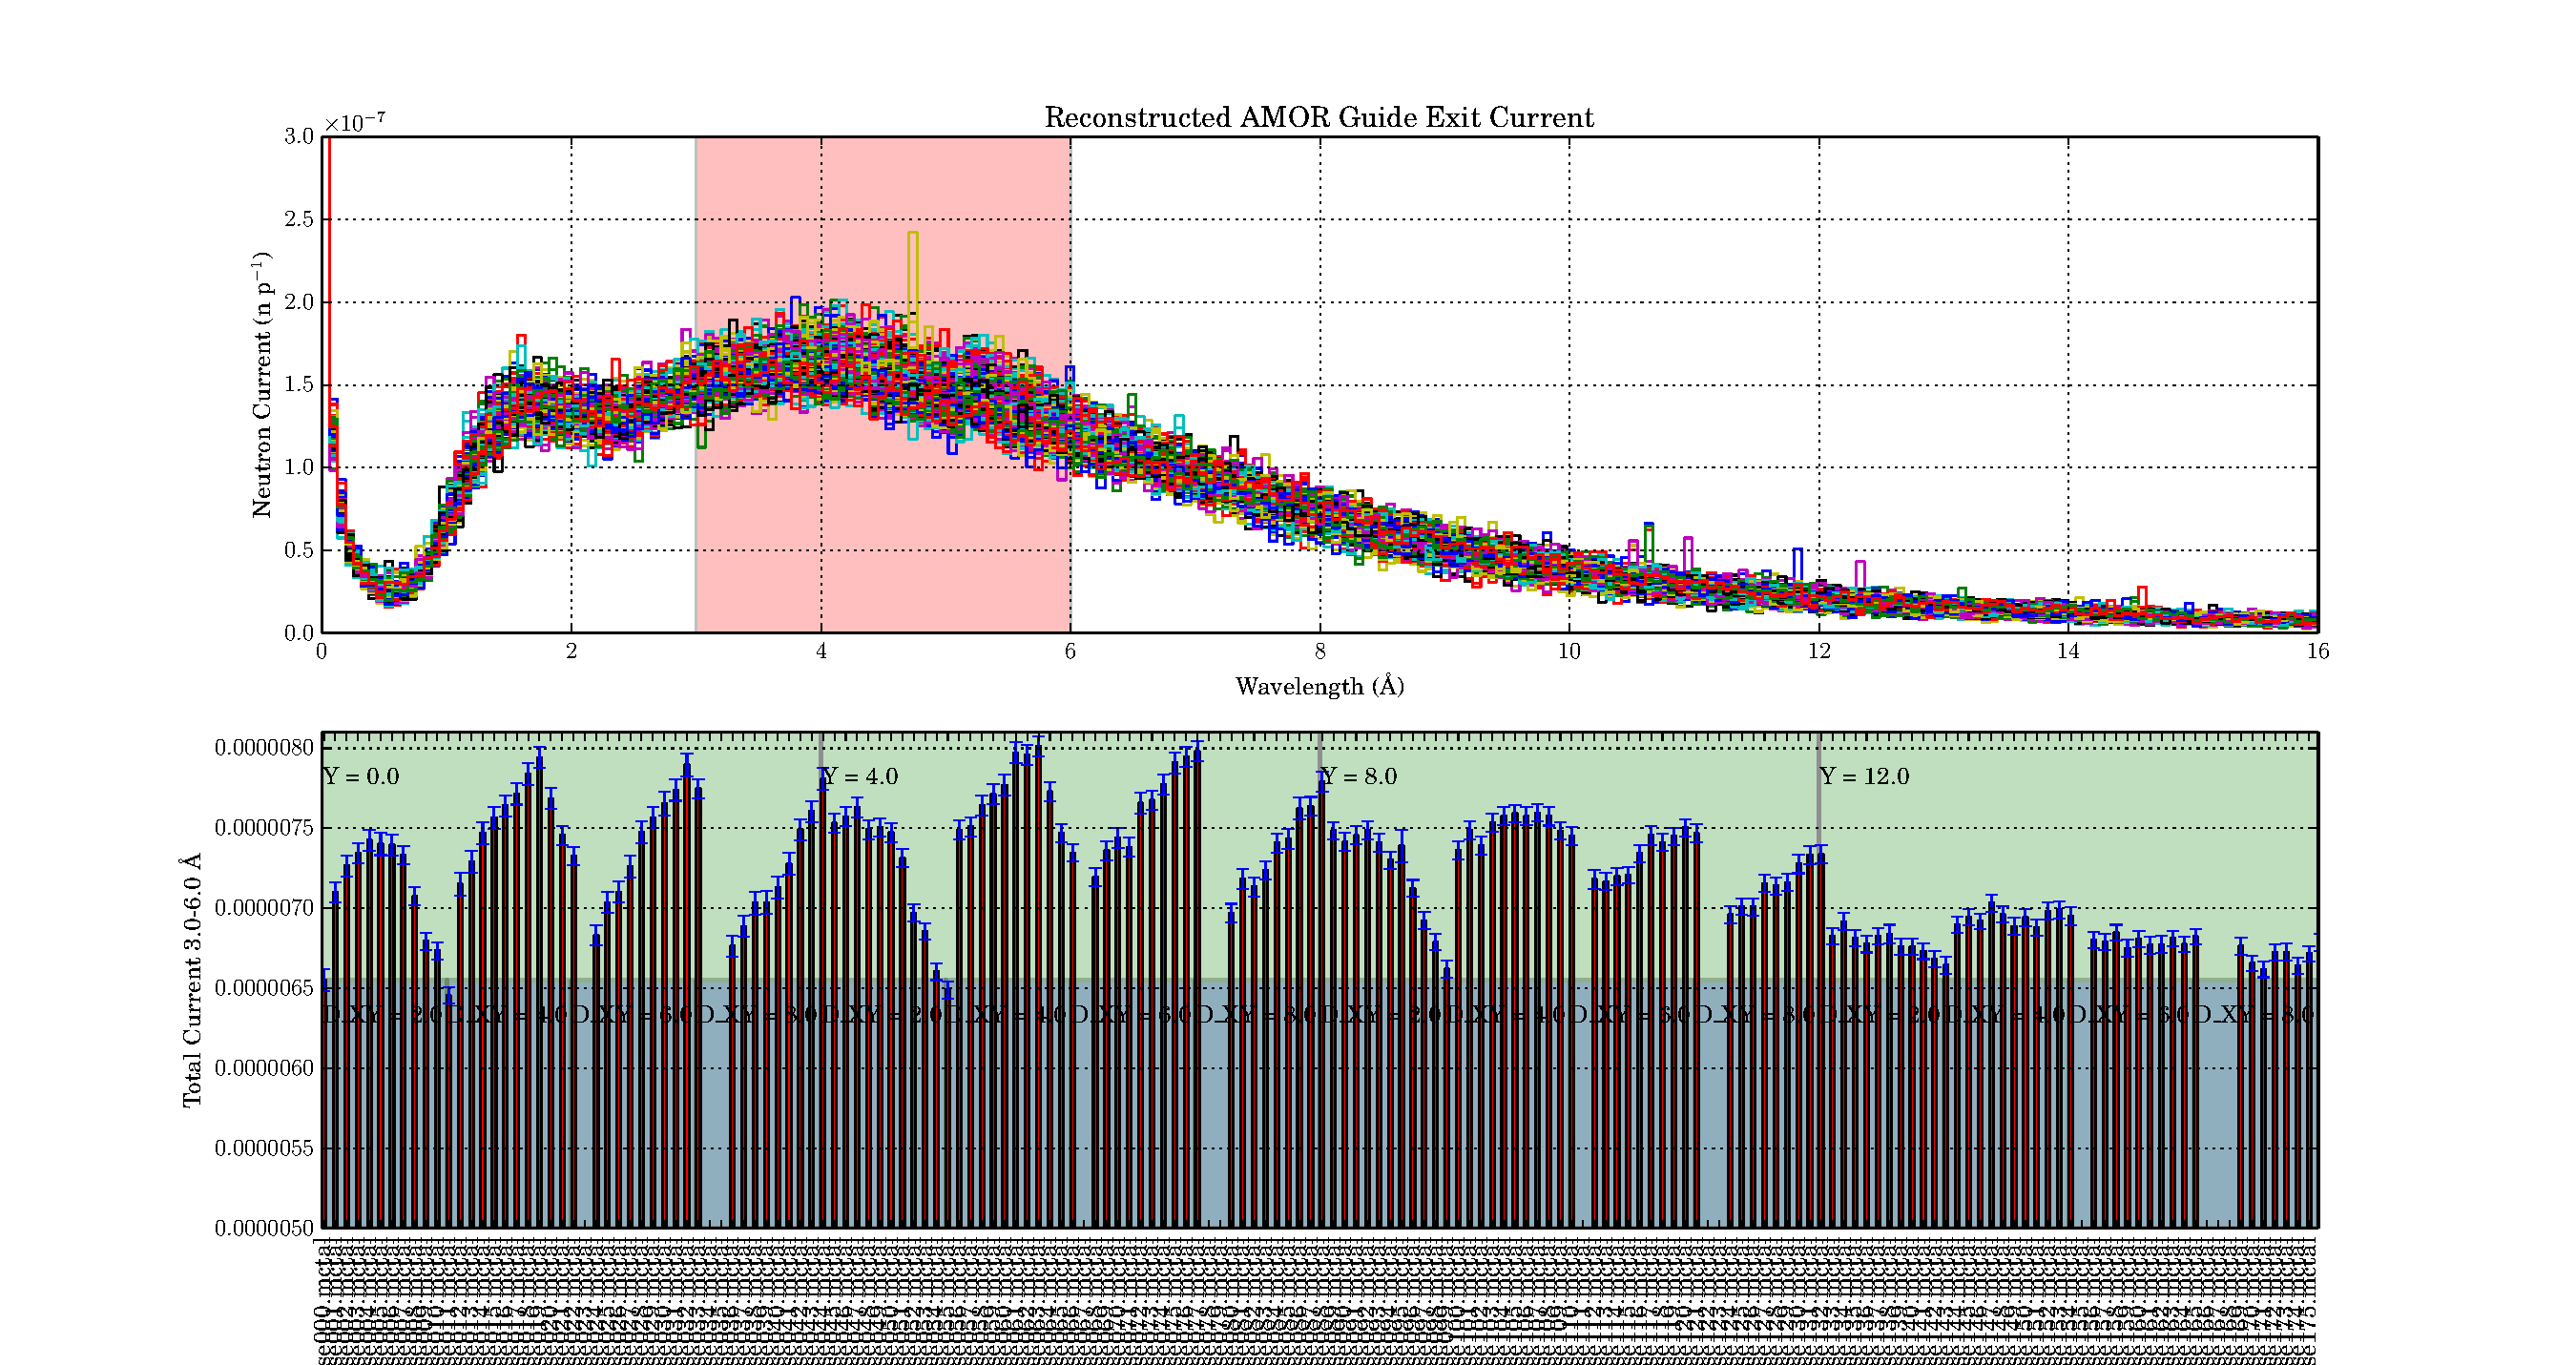
\includegraphics[scale=0.38,trim={1cm 2.35cm 1cm 0cm},clip]{graphics/parametric_REH.pdf}
\end{center}
\caption{\label{parametric_REH}The envelope formed by the spectra from all 176 cases considered (upper) and their figures of merit (lower) which is total current from 3 to 6 \AA{}.}
\end{figure}

\begin{figure}
\begin{center}
\includegraphics[scale=0.38,trim={0cm 0cm 0cm 0cm},clip]{graphics/parametric_gain.pdf}
\end{center}
\caption{\label{parametric_gain}The gain factor of the neutron guide exit current of best-performing REH geometry over the REH being absent.}
\end{figure}


Figure \ref{parametric_gain} shows the gain from the best performaning REH geometry over an absent REH.  The maximum gain 1.32 at 5.5 \AA{} and its average value from 3-6 \AA{} is 1.25.  Similar gains should be seen by all instruments in the SINQ guide hall.  The drop in gain after 5.5 \AA{} is suspected to be from the liquid D$_2$ cross section dropping from about 5.5 to 25 \AA{}, making it more transparent to colder neutrons and reducing the re-entrant hole's benefits.


\section{Conculsions}

From this study and the requirements it imposed on the simulation method, it can be concluded that the flux reconstruction method has been verified to be at least self-consistent, and that a near-optimal horizontal REH geometry has been determined.  The REH increases total exit current by 1.25\% on average from 3-6 \AA{} with a peak gain of 1.32 at 5.5 \AA{}.

\section{Future Work}

This study has only determined the horizontla geometry of the re-entrant hole in the cold source at SINQ.  Another study is needed to investigate REH sensitivity to vertical changes, as well as a parametric study over a smaller range near the optimal point to determine more exact dimensions.  The affect the REH has on the neutron flux on the opposite side will also be determined.

Different types of reflector materials and configurations will also be investigated.  The refector sits behind the cold source on the side opposite the target and reducing cold neutron losses in it may increase the guide exit current.  Adding a belt of liquid H$_2$ to produce a ``cold spot'' for focusing instruments will also be investigated.  In these studies, the flux reconstruction method will once again be used.

Futher development of the guide refelctivity patch for MCNP 6.1 will also be done.  Specifically, making a switch to reduce neutron weight upon reflection instead of leaking non-reflected neutrons in order to speed up in-beam calculations where this signal is of interest and not the noise.

\section*{References}
\bibliography{paper}


\end{document}
